\section{Mathematik 50\% (Lehramt)}

\begin{figure*}[b]
\centering
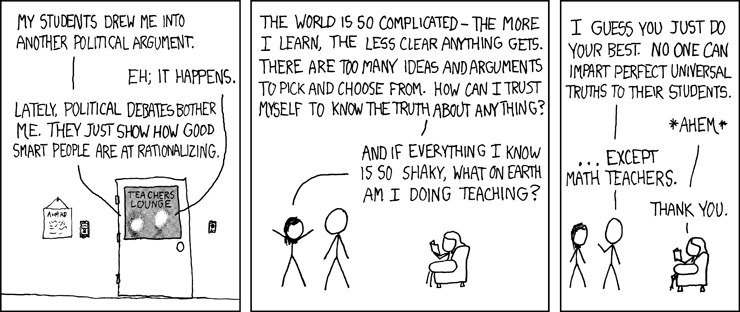
\includegraphics[width=\textwidth]{bilder/certainty.jpg}
\end{figure*}

\subsection{Die ersten Semester}

In der Mathematik startet man mit den Grundvorlesungen \vl{Analysis 1} und \vl{2} und \vl{Lineare Algebra 1} und \vl{2}; jede dieser vier Vorlesungen gibt jeweils 8~\gls{LP}. Die Vorlesungen \gls{Ana}~1 und \gls{LA}~1 finden im Wintersemester, \gls{Ana}~2 und \gls{LA}~2 finden im Sommersemester statt. 

Je nach der Wahl des zweiten Fachs können die ersten beiden Semester damit sehr voll sein. Viele Lehramtsstudierende konzentrieren sich deshalb entweder auf Mathematik und hören nur wenige Vorlesungen aus dem zweiten Fach oder entscheiden sich für eines der beiden Module, also entweder den \vl{Analysis} oder \vl{Lineare Algebra}-Zyklus. Wichtig ist allerdings, dass \gls{LA}~1 die Orientierungsprüfung ist, die ihr bis zum Ende des dritten Semester bestanden haben müsst, sonst dürft ihr nicht weiter studieren.

Solltet ihr aber feststellen, dass euch vier Vorlesungen im ersten Semester zu viel sind, dann ist das kein Weltuntergang. Ihr solltet euch dann entweder ganz auf Mathematik oder nur auf eines der beiden Module \vl{Lineare Algebra} oder \vl{Analysis} konzentrieren. Das kann natürlich dazu führen, dass sich euer Studium um ein oder zwei Semester verlängert. Auch in anderen Bachelor-Studiengängen, zum Beispiel im Mathematik Bachelor 100\%, ist die durchschnittliche Studienzeit höher als die Regelstudienzeit. Wenn ihr länger als die Regelstudienzeit studiert, kann es sein, dass ihr für die zusätzlichen Semester kein BAföG mehr bekommt. Aber auch da gibt es Ausnahmen. Ihr solltet euch, falls ihr Vorlesungen in spätere Semester schiebt, frühzeitig bei den zuständigen Stellen informieren.

\subsection{Wahlpflichtbereich und Seminare}

Nachdem ihr die Grundvorlesungen absolviert habt, könnt ihr euch aussuchen, in welcher Reihenfolge ihr die Vorlesungen aus dem Wahlpflichtbereich hören wollt. Das sind
\begin{itemize}
  \item \vl{Algebra 1}
  \item \vl{Funktionentheorie 1} (\gls{FunkTheo})
  \item \vl{Einführung in die Wahrscheinlichkeitstheorie und Statistik} (\gls{WTheo0})
  \item \vl{Einführung in die Numerik} (\gls{Num0})
\end{itemize}
alle wieder jeweils zu 8~\gls{LP}. 

Im Bachelor müsst ihr mindestens drei der vier zur Wahl stehenden Vorlesungen hören. Dabei müsst ihr beachten, dass ihr am Ende des Master of Education alle vier Wahlpflicht-Vorlesungen bestanden haben müsst. Das heißt, ihr könnt im Bachelor alle vier Wahlpflicht-Vorlesungen hören oder ihr besucht im Bachelor drei Wahlpflichtvorlesungen und eine Veranstaltung aus dem Angebot der Fakultät. Dann belegt ihr die euch noch fehlende Wahlpflicht-Vorlesung im Master. Bei eurer Wahl der Veranstaltung aus dem Angebot der Fakultät ist das Modulhandbuch zum 50\%-Bachelor zu beachten. Falls ihr euch ein Seminar auswählt, solltet ihr auf die Leistungspunkte achten. Da im Allgemeinen ein Seminar nur mit 6 \gls{LP} eingeht, kann es sein, dass die Dozentin beispielsweise eine schriftliche Ausarbeitung oder ähnliches als „Extra“-Leistung für die zusätzlichen 2 \gls{LP} fordert. Hier solltet ihr einfach die Dozentinnen frühzeitig ansprechen.

Außerdem müsst ihr im Bachelor noch jeweils ein \vl{Proseminar} und ein \vl{Seminar} machen; die bringen jeweils 6~\gls{LP}.

\subsection{Fachübergreifende Kompetenzen}

Als fachübergreifende Kompetenzen (FÜK) müsst ihr bildungswissenschaftliche Veranstaltungen belegen, da diese Zulassungsvoraussetzung für den Master of Education sind. Welche genau das sind, findet ihr im Artikel über das allgemeine Lehramt. Damit bleiben euch keine Leistungspunkte im Bereich der FÜK mehr übrig. Beachtet, dass pro Fach bis zu 2 \gls{LP} der insgesamt 20 FÜK-\gls{LP} bereits in den Pflichtvorlesungen euer beiden Studienfächer integriert sind. In \vl{Proseminar} und \vl{Seminar} im Mathematikanteil sind bereits 2 \gls{LP} für Fachdidaktik integriert. Diese zählen sozusagen bildungswissenschaftlich.

\subsection{Bachelor-Arbeit}

Als letztes bleibt noch die Entscheidung zu fällen, in welchem Fach ihr eure Bachelor-Arbeit schreiben wollt. Diese Entscheidung bestimmt, welches euer erstes Hauptfach ist und ob ihr dann mit einem Bachelor of Science oder einen Bachelor of Arts abschließt. In der Mathematik ist es per se leider nur mit bestimmten Fachkombinationen möglich, überhaupt eine Bachelorarbeit in Mathe zu schreiben. Für andere Kombinationen müsst ihr bei der Fakultät einen Antrag stellen, eine Ausnahme sollte aber bei entsprechender Motivation gut machbar sein.

Solltet ihr nach dem Doppelbachelor doch einen Fach-Master machen wollen, ist in den meisten Fächern dann auch die Bachelorarbeit in diesem Fach Zulassungsvoraussetzung für den Fach-Master.